\documentclass[10pt, t, xcolor=dvipsnames]{beamer}

\newcommand\hmmax{0}
\newcommand\bmmax{0}

\usepackage[utf8]{inputenc}
\usepackage[T1]{fontenc}
\usepackage[utopia]{mathdesign}
\usepackage[style=numeric-comp, 
            backend=biber,
            url=false,
            doi=true,
            eprint=false]{biblatex}
\usepackage{subcaption}
\usepackage{graphicx}
\usepackage{relsize}
\usepackage{apacite}
\usepackage{amsmath}
\usepackage{amssymb}
\usepackage{mathtools}
\usepackage{siunitx}
\usepackage{braket}
\usepackage{physics}
\usepackage{tikz}
\usepackage{bm}
\usepackage[usenames,dvipsnames,cmyk]{xcolor}

\setbeamercolor{frametitle}{fg=orange, bg=red!10}
\setbeamercolor{progress bar}{fg=red, bg=red!30}
\setbeamercolor{progress bar in head/foot}{fg=red, bg=red!30}
\setbeamercolor{progress bar in section page}{fg=red, bg=red!30}

\definecolor{filecolor}{RGB}{180,43,190}
\definecolor{funccolor}{RGB}{150,83,210}
\newcommand{\hltexttt}[1]{\texttt{\color{filecolor}{#1}}}
\newcommand{\hltextttf}[1]{\texttt{\color{funccolor}{#1}}}
  
\usetikzlibrary{arrows.meta, shadows}

\addbibresource{text/refs.bib}

\usetheme[progressbar=frametitle]{metropolis}
\usepackage{appendixnumberbeamer}

\usepackage{booktabs}
\usepackage[scale=2]{ccicons}

\usepackage{pgfplots}
\usepgfplotslibrary{dateplot}

\usepackage{xspace}
\newcommand{\themename}{\textbf{\textsc{metropolis}}\xspace}

\newcommand{\onefigure}[4]{
    \begin{figure}[H]
        \centering
        \textbf{{#1}}\\
        \includegraphics[scale=0.95]{{#2}}
        \caption{{#3}}
        \label{fig:#4}
    \end{figure}
    \justifying
} %one figure {filename}{caption}
\newcommand{\twofigure}[2]{
    \begin{figure}[H]
        \centering
        \begin{subfigure}[b!]{0.49\textwidth}
            \centering
            \includegraphics[width=\textwidth]{{#1}}
        \end{subfigure}
        \begin{subfigure}[b!]{0.49\textwidth}
            \centering
            \includegraphics[width=\textwidth]{{#2}}
        \end{subfigure}
        \justify
    \end{figure}
} %two figure one-line {title}{file1}{caption1}{file2}{caption2}

\title{Quantum Many-Body Simulations of Double Dot System}
% \date{\today}
\date{}
\author{Alocias Mariadason}
\institute{Institute of Physics}
% \titlegraphic{\hfill\includegraphics[height=1.5cm]{logo.pdf}}

\newcommand{\prtl}{\mathrm{\partial}} %reduce length of partial (less to write)
\NewDocumentCommand{\prd}{m O{} O{}}{\frac{\prtl^{#3}{#2}}{\prtl{#1}^{#3}}}
\newcommand{\prdp}[2]{\left(\frac{\prtl}{\prtl #1}\right)^{#2}}
\newcommand{\vsp}{\vspace{0.2cm}} %small vertical space
\newcommand{\txtit}[1]{\textit{{#1}}} %italic text
\newcommand{\blds}[1]{\boldsymbol{{#1}}} % better bold in mathmode (from amsmath)
\newcommand{\bigO}{\mathcal{O}} %nice big O
\newcommand{\me}{\mathrm{e}} %straight e for exp
\newcommand{\md}{\mathrm{d}} %straight d for differential
\newcommand{\mRe}[1]{\mathrm{Re}\left({#1}\right)}%nice real
\newcommand{\munit}[1]{\;\ensuremath{\, \mathrm{#1}}} %straight units in math
\newcommand{\Rarr}{\Rightarrow} %reduce lenght of Rightarrow (less to write)
\newcommand{\rarr}{\rightarrow} %reduce lenght of rightarrow (less to write)
\newcommand{\ecp}[1]{\left< {#1} \right>} %expected value
\newcommand{\urw}{\uparrow} % up arrow
\newcommand{\drw}{\downarrow} % up arrow
\newcommand{\pt}[1]{\textbf{\txtit{#1}}\justify}
\newcommand{\infint}{\int\limits^{\infty}_{-\infty}}
\newcommand{\oinfint}{\int\limits^{\infty}_0}
\newcommand{\sint}{\int\limits^{2\pi}_0\int\limits^{\pi}_0\oinfint}
\newcommand{\arcsinh}[1]{\text{arcsinh}\left(#1\right)}
\newcommand{\I}{\scalebox{1.2}{$\mathds{1}$}}
\newcommand{\veps}{\varepsilon} %\varepsilon is to long :P
\newcommand{\cnj}[1]{{#1}^{*}}
\newcommand{\Arf}[1]{\Autoref{#1}}

\newcommand{\ufij}[3]{#1_{#2\rarr#3}}
\newcommand{\Ham}{\hat{H}}
\newcommand{\mb}[1]{\blds{#1}}
\newcommand{\psiTcnj}{\cnj{\Psi}_T(\mb{R};\mb{\alpha})}
\newcommand{\psiT}{{\Psi}_T(\mb{R};\mb{\alpha})}
\newcommand{\dinner}[2]{\bra{#1}#2\ket{#1}}
\newcommand{\pinner}{\dinner{\Psi_T}{}}
\newcommand{\langevin}{\prd{t}[r] = DF(r(t)) + \eta}
\newcommand{\rnew}{r^{\text{new}}}
\newcommand{\rold}{r^{\text{old}}}
\newcommand{\Fnew}{F^{\text{new}}}
\newcommand{\Fold}{F^{\text{old}}}
\newcommand{\FokkerPlanck}{\prd{t}[P] = \sum_i D\prd{x_i}\left(\prd{x_i} - \mb{F_i}\right)P}
\newcommand{\Kin}{\frac{1}{2}\sum_i\nabla^2_i}
\newcommand{\frij}{f(\blds{r}_i, \blds{r}_j)}
\newcommand{\fij}{f_{ij}}
\newcommand{\HO}{V(\blds{R}) - \Kin}
\newcommand{\HI}{\sum\limits_{i<j} \frij}
\newcommand{\EHF}{E\left[\Psi^{\text{HF}}\right]}
\newcommand{\HIinnerAS}[2]{\bra{\psi_{#1}\psi_{#2}}H_I\ket{\psi_{#1}\psi_{#2}} - \bra{\psi_{#1}\psi_{#2}}H_I\ket{\psi_{#2}\psi_{#1}}}

\newcommand{\ijnorm}[2]{\sqrt{\braket{#1}{#1}\braket{#2}{#2}}}


\begin{document}

\maketitle

\begin{frame}{Contents}
  \setbeamertemplate{section in toc}[sections numbered]
  \tableofcontents[hideallsubsections]
\end{frame}

\section{Introduction}

\begin{frame}[fragile]{Quantum-Dot}
    \begin{itemize}
        \item Small semiconductor nanostructures
        \item $2$-$10$ nanometers with $10-50$ particles
    \end{itemize}
\end{frame}

\begin{frame}[fragile]{Quantum-Dot Model}
    \begin{itemize}
        \item Schrödinger equation 
            \begin{itemize}
                \item $\mathcal{H}\ket{\psi} = E\ket{\psi}$
            \end{itemize}
    \end{itemize}
\end{frame}

\begin{frame}[fragile]{Quantum-Dot Model}
    \begin{itemize}
        \item Schrödinger equation 
            \begin{itemize}
                \item $\mathcal{H}\ket{\psi} = E\ket{\psi}$
            \end{itemize}
        \item Hamiltonian
            \begin{itemize}
                \item $\mathcal{H} = - \frac{1}{2} \sum\limits_i \nabla^2_i +
                    \sum\limits_{i<j} f\left(\blds{r}_j, \blds{r}_j\right) -
                    \frac{1}{2} \sum\limits_k \frac{\nabla^2_k}{M_k} + \sum\limits_{k<l}
                    g\left(\blds{R}_k,\blds{R}_l\right) +
                    V\left(\blds{R},\blds{r}\right)$
            \end{itemize}
    \end{itemize}
\end{frame}

\begin{frame}[fragile]{Quantum-Dot Model}
    \begin{itemize}
        \item Schrödinger equation 
            \begin{itemize}
                \item $\mathcal{H}\ket{\psi} = E\ket{\psi}$
            \end{itemize}
        \item Hamiltonian
            \begin{itemize}
                \item $\mathcal{H} = - \frac{1}{2} \sum\limits_i \nabla^2_i +
                    \sum\limits_{i<j} f\left(\blds{r}_j, \blds{r}_j\right) -
                    \frac{1}{2} \sum\limits_k \frac{\nabla^2_k}{M_k} + \sum\limits_{k<l}
                    g\left(\blds{R}_k,\blds{R}_l\right) +
                    V\left(\blds{R},\blds{r}\right)$
            \end{itemize}
        \item Born-Oppenheimer Approximation
            \begin{itemize}
                \item Ignore Nuclei
                \item $\sum\limits_k \frac{\nabla^2_k}{M_k}$ gone
                \item $\sum\limits_{k<l} g\left(\blds{R}_k,\blds{R}_l\right)$ constant
            \end{itemize}
    \end{itemize}
\end{frame}

\begin{frame}[fragile]{Quantum-Dot Model}
    \begin{itemize}
        \item Schrödinger equation 
            \begin{itemize}
                \item $\mathcal{H}\ket{\psi} = E\ket{\psi}$
            \end{itemize}
        \item Hamiltonian
            \begin{itemize}
                \item $\mathcal{H} = - \frac{1}{2} \sum\limits_i \nabla^2_i +
                    \sum\limits_{i<j} f\left(\blds{r}_j, \blds{r}_j\right) -
                    \frac{1}{2} \sum\limits_k \frac{\nabla^2_k}{M_k} + \sum\limits_{k<l}
                    g\left(\blds{R}_k,\blds{R}_l\right) +
                    V\left(\blds{R},\blds{r}\right)$
            \end{itemize}
        \item Born-Oppenheimer Approximation
            \begin{itemize}
                \item Ignore Nuclei
                \item $\sum\limits_k \frac{\nabla^2_k}{M_k}$ gone
                \item $\sum\limits_{k<l} g\left(\blds{R}_k,\blds{R}_l\right)$ constant
                \item $\mathcal{H} = - \frac{1}{2} \sum\limits_i \nabla^2_i +
                    \sum\limits_{i<j} f\left(\blds{r}_j, \blds{r}_j\right) +
                    V\left(\blds{R},\blds{r}\right)$
            \end{itemize}
    \end{itemize}
\end{frame}

\begin{frame}[fragile]{Quantum-Dot Model}
    \begin{itemize}
        \item Interaction
            \begin{itemize}
                \item $f\left(\blds{r}_i, \blds{r}_j\right) =
                    \frac{1}{\abs{\blds{r}_i - \blds{r}_j}}$
            \end{itemize}
    \end{itemize}
\end{frame}

\begin{frame}[fragile]{Quantum-Dot Model}
    \centering
    \begin{itemize}
        \item Interaction: Coulomb repulsion
            \begin{itemize}
                \item $f\left(\blds{r}_i, \blds{r}_j\right) =
                    \frac{1}{\abs{\blds{r}_i - \blds{r}_j}}$
            \end{itemize}
        \item Confinement: Harmonic Oscillator\footfullcite{kvaaldots}, Double-Well\footfullcite{ddotnuc}
    \end{itemize}
    \vspace{-0.2cm}
    \begin{align*}
        V(\blds{r}) = \frac{1}{2} \omega mr^2& \hspace{1cm}
        &V(\blds{R},\blds{r}) = \frac{1}{2}m\omega^2\left(r^2 - \delta R\abs{x}
        + R^2\right)
    \end{align*}
    \vspace{-0.80cm}
    \twofigure{text/figs/HO2Dplot.pdf}{text/figs/DW2Dplot.pdf}
\end{frame}

\section{Methods}

{\setbeamercolor{palette primary}{fg=black, bg=white}
\begin{frame}[standout]{Methods}
    Hartree-Fock \\
    Variational Monte-Carlo
\end{frame}

{\setbeamercolor{palette primary}{fg=black, bg=white}
\begin{frame}[standout]{Methods: Variational Principle}
    \begin{equation*}
        E_0 \leq \frac{\Braket{\Psi|\mathcal{H}|\Psi}}{\Braket{\Psi|\Psi}}
        \label{eq:varPrinc}
    \end{equation*}
\end{frame}

\begin{frame}[fragile]{Methods: Slater Determinant and Energy Functional}
    \begin{itemize}
        \item Pauli Principle
    \end{itemize}
\end{frame}

\begin{frame}[fragile]{Methods: Slater Determinant and Energy Functional}
    \begin{itemize}
        \item Pauli Principle
        \item Slater Determinant
            \begin{itemize}
                \item $\Psi^{\text{AS}}_T =
                    \frac{1}{\sqrt{N!}}\sum\limits_{P}(-1)^p\mathcal{P}_P\prod\limits_i\psi_i$
                \item $\Psi^{\text{S}}_T =
                    \sqrt{\frac{\prod\limits^N_{i=1}n_i!}{N!}}\sum\limits_{P}\mathcal{P}_P\prod\limits_i\psi_i$
            \end{itemize}
    \end{itemize}
\end{frame}

\begin{frame}[fragile]{Methods: Slater Determinant and Energy Functional}
    \begin{itemize}
        \item Pauli Principle
        \item Slater Determinant
            \begin{itemize}
                \item $\Psi^{\text{AS}}_T =
                    \frac{1}{\sqrt{N!}}\sum\limits_{P}(-1)^p\mathcal{P}_P\prod\limits_i\psi_i$
                \item $\Psi^{\text{S}}_T =
                    \sqrt{\frac{\prod\limits^N_{i=1}n_i!}{N!}}\sum\limits_{P}\mathcal{P}_P\prod\limits_i\psi_i$
            \end{itemize}
        \item $E\left[\Psi\right] =
            \frac{\Braket{\Psi|\mathcal{H}|\Psi}}{\Braket{\Psi|\Psi}} =
            \sum\limits_p\bra{p}\mathcal{H}_0\ket{p} +
            \frac{1}{2}\sum\limits_{p,q}\left[\bra{pq}f_{12}\ket{pq} \pm
            \bra{pq}f_{12}\ket{qp}\right]$
        \item $\mathcal{H}_0 = -\frac{1}{2}\sum\limits_i\nabla^2_i + V(r)$
    \end{itemize}
\end{frame}

\begin{frame}[fragile]{Methods: Hartree-Fock}
    \begin{itemize}
        \item Assumptions
        \begin{itemize}
            \item The Born-Oppenheimer approximation holds. 
            \item All relativistic effects are negligible.
            \item The wavefunction can be described by a single \txtit{Slater
                determinant}.
            \item The Mean Field Approximation holds.
        \end{itemize}
    \end{itemize}
\end{frame}

\begin{frame}[fragile]{Methods: Hartree-Fock}
    \begin{itemize}
        \item Assumptions
        \begin{itemize}
            \item The Born-Oppenheimer approximation holds. 
            \item All relativistic effects are negligible.
            \item The wavefunction can be described by a single \txtit{Slater
                determinant}.
            \item The Mean Field Approximation holds.
        \end{itemize}
    \end{itemize}
    \begin{figure}[H]
        \centering
        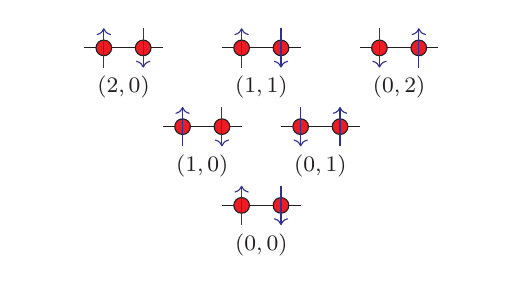
\begin{tikzpicture}[scale=0.5]
            \draw (-1,0) -- (1,0);
            \node at (-0.5,0) [draw,circle,fill=red,scale=0.6] {};
            \node at (0.5,0) [draw,circle,fill=red,scale=0.6] {};
            \draw[blue, ->] (-0.5,-0.5) -- (-0.5,0.5);
            \draw[blue, <-] (0.5,-0.5) -- (0.5,0.5);
            \node[text width=2.2cm, align=center] at (0,-1) {\footnotesize{$(0,0)$}};
            \draw (-2.5,2) -- (-0.5,2);
            \node at (-2.0,2) [draw,circle,fill=red,scale=0.6] {};
            \node at (-1.0,2) [draw,circle,fill=red,scale=0.6] {};
            \draw[blue, ->] (-2.0,1.5) -- (-2.0,2.5);
            \draw[blue, <-] (-1.0,1.5) -- (-1.0,2.5);
            \node[text width=2.2cm, align=center] at (-1.5,1) {\footnotesize{$(1,0)$}};
            \draw (0.5,2) -- (2.5,2);
            \node at (1.0,2) [draw,circle,fill=red,scale=0.6] {};
            \node at (2.0,2) [draw,circle,fill=red,scale=0.6] {};
            \draw[blue, <-] (1.0,1.5) -- (1.0,2.5);
            \draw[blue, ->] (2.0,1.5) -- (2.0,2.5);
            \node[text width=2.2cm, align=center] at (1.5,1) {\footnotesize{$(0,1)$}};
            \draw (-4.5,4) -- (-2.5,4);
            \node at (-4.0,4) [draw,circle,fill=red,scale=0.6] {};
            \node at (-3.0,4) [draw,circle,fill=red,scale=0.6] {};
            \draw[blue, ->] (-4.0,3.5) -- (-4.0,4.5);
            \draw[blue, <-] (-3.0,3.5) -- (-3.0,4.5);
            \node[text width=2.2cm, align=center] at (-3.5,3) {\footnotesize{$(2,0)$}};
            \draw (-1,4) -- (1,4);
            \node at (-0.5,4) [draw,circle,fill=red,scale=0.6] {};
            \node at (0.5,4) [draw,circle,fill=red,scale=0.6] {};
            \draw[blue, ->] (-0.5,3.5) -- (-0.5,4.5);
            \draw[blue, <-] (0.5,3.5) -- (0.5,4.5);
            \node[text width=2.2cm, align=center] at (0,3) {\footnotesize{$(1,1)$}};
            \draw (4.5,4) -- (2.5,4);
            \node at (4.0,4) [draw,circle,fill=red,scale=0.6] {};
            \node at (3.0,4) [draw,circle,fill=red,scale=0.6] {};
            \draw[blue, ->] (4.0,3.5) -- (4.0,4.5);
            \draw[blue, <-] (3.0,3.5) -- (3.0,4.5);
            \node[text width=2.2cm, align=center] at (3.5,3) {\footnotesize{$(0,2)$}};
        \end{tikzpicture}
    \end{figure}
\end{frame}

\begin{frame}[fragile]{Methods: Hartree-Fock}
    \begin{itemize}
        \item Constrained minimization
    \end{itemize}
\end{frame}

\begin{frame}[fragile]{Methods: Hartree-Fock}
    \begin{itemize}
        \item Constrained minimization
            \begin{itemize}
                \item Spin orthogonality: $\braket{\psi_i}{\psi_j} =
                    \delta_{ij}$
            \end{itemize}
    \end{itemize}
\end{frame}

\begin{frame}[fragile]{Methods: Hartree-Fock}
    \begin{itemize}
        \item Constrained minimization
            \begin{itemize}
                \item Spin orthogonality: $\braket{\psi_i}{\psi_j} =
                    \delta_{ij}$
                \item Lagrange Multiplier method
            \end{itemize}
    \end{itemize}
\end{frame}

\begin{frame}[fragile]{Methods: Hartree-Fock}
    \begin{itemize}
        \item Constrained minimization
            \begin{itemize}
                \item Spin orthogonality: $\braket{\psi_i}{\psi_j} =
                    \delta_{ij}$
                \item Lagrange Multiplier method
                \item Fock-operator: $\mathcal{F} \equiv \mathcal{H}_0 +
                    \mathcal{J} \pm \mathcal{K}$
                    \begin{itemize}
                        \item $\mathcal{J} \equiv
                            \bra{\psi^{*}_k}f_{12}\ket{\psi_k} = \int
                            \psi^{*}_k(\blds{r})f_{12}\psi_k(\blds{r})\md r$
                        \vsp
                        \item $\mathcal{K} \equiv
                            \bra{\psi^{*}_k}f_{12}\ket{\psi} = \int
                            \psi^{*}_k(\blds{r})f_{12}\psi(\blds{r})\md r$
                        \vsp
                        \item $\mathcal{F}\ket{\psi} = \blds{\veps}\ket{\psi},
                            \blds{\veps}=(\veps_0,\dots,\veps_N)$
                    \end{itemize}
            \end{itemize}
    \end{itemize}
\end{frame}

\begin{frame}[fragile]{Methods: Hartree-Fock}
    \begin{itemize}
        \item Constrained minimization
            \begin{itemize}
                \item Spin orthogonality: $\braket{\psi_i}{\psi_j} =
                    \delta_{ij}$
                \item Lagrange Multiplier method
                \item Fock-operator: $\mathcal{F} \equiv \mathcal{H}_0 + \mathcal{J} \pm \mathcal{K}$
                    \begin{itemize}
                        \item $\mathcal{J} \equiv
                            \bra{\psi^{*}_k}f_{12}\ket{\psi_k} = \int
                            \psi^{*}_k(\blds{r})f_{12}\psi_k(\blds{r})\md r$
                        \vsp
                        \item $\mathcal{K} \equiv
                            \bra{\psi^{*}_k}f_{12}\ket{\psi} = \int
                            \psi^{*}_k(\blds{r})f_{12}\psi(\blds{r})\md r$
                        \vsp
                        \item $\mathcal{F}\ket{\psi} = \blds{\veps}\ket{\psi},
                            \blds{\veps}=(\veps_0,\dots,\veps_N)$
                    \end{itemize}
                \item $N+1$ equations to be solved.
            \end{itemize}
    \end{itemize}
\end{frame}

\begin{frame}[fragile]{Methods: Hartree-Fock}
    \begin{itemize}
        \item Integrate out spin
        \item Pair spins as: $\{\psi_{2l-1}, \psi_{2l}\} =
            \{\phi_l(\blds{r})\alpha(s),\phi_l(\blds{r})\beta(s)\}$
    \end{itemize}
\end{frame}

\begin{frame}[fragile]{Methods: Hartree-Fock}
    \begin{itemize}
        \item Integrate out spin
        \item Pair spins as: $\{\psi_{2l-1}, \psi_{2l}\} =
            \{\phi_l(\blds{r})\alpha(s),\phi_l(\blds{r})\beta(s)\}$
        \item Expand: $\phi_i(\blds{r}) = \sum\limits^L_{p=1} C_{pi}\chi_p(\blds{r})$
    \end{itemize}
\end{frame}

\begin{frame}[fragile]{Methods: Hartree-Fock}
    \begin{itemize}
        \item Integrate out spin
        \item Pair spins as: $\{\psi_{2l-1}, \psi_{2l}\} =
            \{\phi_l(\blds{r})\alpha(s),\phi_l(\blds{r})\beta(s)\}$
        \item Expand: $\phi_i(\blds{r}) = \sum\limits^L_{p=1} C_{pi}\chi_p(\blds{r})$
        \item Roothan-Hall: $\blds{F}\blds{C}_i = \blds{\veps}S\blds{C}_i$
            \begin{itemize}
                \item $F_{pq} = h_{pq} + \sum\limits_{pq}\rho_{pq}\left(2D_{prqs} \pm D_{prsq}\right)$
                \vsp
                \item $h_{pq} \equiv \Braket{p | h | q}$
                \vsp
                \item $\rho_{pq} \equiv \sum\limits^{\frac{N}{2}}_{i=1} C_{pi}C^{*}_{qi}$
                \vsp
                \item $D_{pqrs} \equiv \Braket{pq | f_{12} | rs}$
                \item $S_{pq} \equiv \Braket{p | q}$
            \end{itemize}
        \item Poople-Nesbet: $\blds{F}^{+}\blds{C}^{+} =
            \blds{\veps}^{\+}\blds{S}\blds{C}^{+}$, $\blds{F}^{-}\blds{C}^{-} =
            \blds{\veps}^{-}\blds{S}\blds{C}^{-}$
            \begin{itemize}
                \item $F^{\pm}_{pq} = h_{pq} + \sumll{k_{\pm}}\sumll{rs}
                    C^{\pm\dagger}_{rk_{\pm}} C^{\pm\dagger}_{sk_{\pm}}
                    \left[D_{prqs} - D_{prsq}\right] +
                    \sumll{k_{\mp}}\sumll{rs} C^{\mp\dagger}_{rk_{\mp}}
                    C^{\mp\dagger}_{sk_{\mp}} D_{prqs}$
            \end{itemize}
    \end{itemize}
\end{frame}

\begin{frame}[fragile]{Methods: Hartree-Fock}
        \begin{figure}
            \centering
            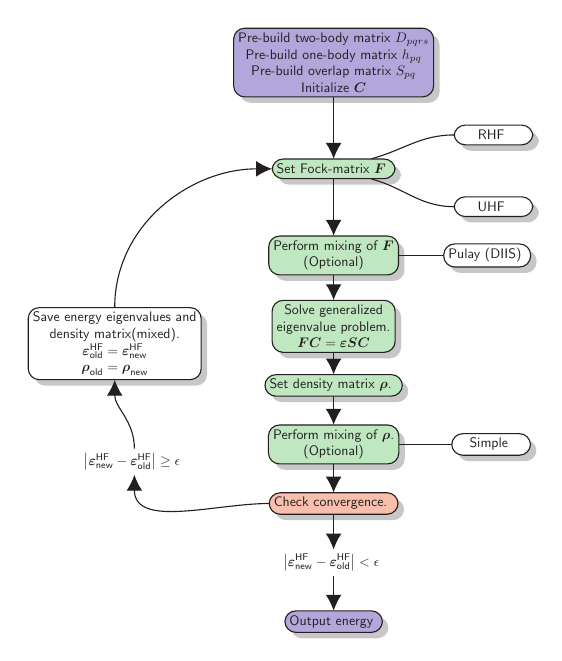
\begin{tikzpicture}[
                >={Latex[width=2mm,length=2mm]},
                    base/.style = {rectangle, rounded corners, draw=black,
                                minimum width=2cm, minimum height=0.5cm, text
                                centered, font=\sffamily},
                    basecode/.style = {rectangle, rounded corners, draw=black,
                                minimum width=2cm, minimum height=0.5cm, text
                                centered, font=\sffamily, align=left},
                    activityStarts/.style = {base, fill=blue!30, drop shadow},
                    startstop/.style = {base, fill=red!25, drop shadow},
                    startstopcode/.style = {basecode, fill=red!25, drop shadow},
                    activityRuns/.style = {base, fill=green!25, drop shadow},
                    process/.style = {base, fill=white!15, font=\sffamily, drop shadow},
                    processcode/.style = {basecode, fill=white!15, font=\sffamily, drop shadow},
                scale=0.5, 
                node distance=1.5cm, 
                every node/.style={fill=white, font=\sffamily, scale=0.5},
                align=center]
                \node (pre) [activityStarts] {
                    Pre-build two-body matrix $D_{pqrs}$ \\
                    Pre-build one-body matrix $h_{pq}$ \\
                    Pre-build overlap matrix $S_{pq}$ \\
                    Initialize $\blds{C}$
                };
                \node (Fock) [activityRuns, below of=pre, yshift=-1.2cm] {
                    Set Fock-matrix $\blds{F}$
                };
                \node (Fockmix) [activityRuns, below of=Fock, yshift=-0.7cm] {
                    Perform mixing of $\blds{F}$ \\
                    (Optional)
                };
                \node (Fockmixeq) [process, right of=Fockmix, xshift=2.4cm] {
                    Pulay (DIIS)
                };
                \draw[->] (Fock) -- (Fockmix);
                \draw[-] (Fockmix) -- (Fockmixeq);
                \node (RHF) [process, above right of=Fock, xshift=3.0cm, yshift=-0.2cm] {
                    RHF
                };
                \node (UHF) [process, below right of=Fock, xshift=3.0cm, yshift=0.1cm] {
                    UHF
                };
                \draw[-] (Fock) to [out=15, in=180] (RHF);
                \draw[-] (Fock) to [out=-15, in=180] (UHF);
                \draw[->] (pre) -- (Fock);
                \node (eigcomp) [activityRuns, below of=Fock, yshift=-2.5cm] {
                    Solve generalized \\ 
                    eigenvalue problem. \\
                    $\blds{F}\blds{C} = \blds{\veps}\blds{S}\blds{C}$
                };
                \draw[->] (Fockmix) -- (eigcomp);
                \node (density) [activityRuns, below of=eigcomp] {
                   Set density matrix $\blds{\rho}$.
                };
                \draw[->] (eigcomp) -- (density);
                \node (mix) [activityRuns, below of=density] {
                    Perform mixing of $\blds{\rho}$. \\
                    (Optional)
                };
                \draw[->] (density) -- (mix);
                \node (mixeq) [process, right of=mix, xshift=2.5cm] {
                    Simple
                };
                \draw[-] (mix) -- (mixeq);
                \node (conv) [startstop, below of=mix] {
                    Check convergence.
                };
                \draw[->] (mix) -- (conv);
                \node (no) [above left of=conv, xshift=-4.0cm] {
                    $\abs{\blds{\varepsilon}^{\text{HF}}_{\text{new}} -
                    \blds{\varepsilon}^{\text{HF}}_{\text{old}}} \geq \epsilon$
                };
                \draw[->] (conv) to [out=180,in=-90] (no);
                \node (keepOld) [process, above of=no, yshift=1.5cm, xshift=-0.5cm] {
                    Save energy eigenvalues and \\
                    density matrix(mixed). \\
                    $\blds{\varepsilon}^{\text{HF}}_{\text{old}} =
                    \blds{\varepsilon}^{\text{HF}}_{\text{new}}$ \\
                    $\blds{\rho}_{\text{old}} = \blds{\rho}_{\text{new}}$
                };
                \draw[->] (no) to [out=90,in=-90] (keepOld);
                \draw[->] (keepOld) to [out=90,in=180] (Fock);
                \node (yes) [below of=conv] {
                    $\abs{\blds{\varepsilon}^{\text{HF}}_{\text{new}} -
                    \blds{\varepsilon}^{\text{HF}}_{\text{old}}} < \epsilon$
                };
                \draw[->] (conv) -- (yes);
                \node (end) [activityStarts, below of=yes] {
                    Output energy
                };
                \draw[->] (yes) -- (end);
            \end{tikzpicture}
        \end{figure}
\end{frame}

\begin{frame}[fragile]{Methods: Variational Monte-Carlo}
    \begin{itemize}
        \item Variational Principle
    \end{itemize}
\end{frame}

\begin{frame}[fragile]{Methods: Variational Monte-Carlo}
    \begin{itemize}
        \item Variational Principle
        \item Rewrite expectation value:
            $\frac{\Braket{\Psi|\mathcal{H}|\Psi}}{\Braket{\Psi|\Psi}} = \int
            \frac{\cnj{\Psi}\mathcal{H}\Psi}{\int \cnj{\Psi}\Psi \md r} \md r
            = \int \frac{\abs{\Psi}^2E_L}{\int \cnj{\Psi}\Psi \md r} \md r$
            \begin{itemize}
                \item $E_L(\mb{R};\mb{\alpha}) \equiv \frac{1}{\Psi}\mathcal{H}\Psi$
                \item $P(\mb{R}) \equiv \frac{\abs{\psi_T}^2}{\pinner}$
            \end{itemize}
    \end{itemize}
\end{frame}

\begin{frame}[fragile]{Methods: Variational Monte-Carlo}
    \begin{itemize}
        \item Variational Principle
        \item Rewrite expectation value:
            $\frac{\Braket{\Psi|\mathcal{H}|\Psi}}{\Braket{\Psi|\Psi}} = \int
            \frac{\cnj{\Psi}\mathcal{H}\Psi}{\int \cnj{\Psi}\Psi \md r} \md r
            = \int \frac{\abs{\Psi}^2E_L}{\int \cnj{\Psi}\Psi \md r} \md r$
            \begin{itemize}
                \item $E_L(\mb{R};\mb{\alpha}) \equiv \frac{1}{\Psi}\mathcal{H}\Psi$
                \item $P(\mb{R}) \equiv \frac{\abs{\psi_T}^2}{\pinner}$
            \end{itemize}
        \item Metropolis-Hastings Algorithm
            \begin{itemize}
                \item $r^{\text{new}} = r^{\text{old}} + \Delta t \xi$
                \item $\ufij{A}{i}{j} =
                    \text{min}\left(\frac{\ufij{P}{i}{j}}{\ufij{P}{j}{i}}
                    \frac{\ufij{T}{i}{j}}{\ufij{T}{j}{i}} ,1\right)$
            \end{itemize}
    \end{itemize}
\end{frame}

\begin{frame}[fragile]{Methods: Variational Monte-Carlo}
    \begin{itemize}
        \item Variational Principle
        \item Rewrite expectation value:
            $\frac{\Braket{\Psi|\mathcal{H}|\Psi}}{\Braket{\Psi|\Psi}} = \int
            \frac{\cnj{\Psi}\mathcal{H}\Psi}{\int \cnj{\Psi}\Psi \md r} \md r
            = \int \frac{\abs{\Psi}^2E_L}{\int \cnj{\Psi}\Psi \md r} \md r$
            \begin{itemize}
                \item $E_L(\mb{R};\mb{\alpha}) \equiv \frac{1}{\Psi}\mathcal{H}\Psi$
                \item $P(\mb{R}) \equiv \frac{\abs{\psi_T}^2}{\pinner}$
            \end{itemize}
        \item Metropolis-Hastings Algorithm
            \begin{itemize}
                \item $r^{\text{new}} = r^{\text{old}} + \Delta t \xi$
                \item $\ufij{A}{i}{j} =
                    \text{min}\left(\frac{\ufij{P}{i}{j}}{\ufij{P}{j}{i}}
                    \frac{\ufij{T}{i}{j}}{\ufij{T}{j}{i}} ,1\right)$
                \item Importance Sampling
                    \begin{itemize}
                        \item $r^{\text{new}} = r^{\text{old}} + D \Delta t
                            F^{\text{old}} + \sqrt{\Delta t}\xi$
                        \item $F = \frac{2}{\Psi}\nabla \Psi$ 
                        \item $\frac{T(b,a,\Delta t)}{T(a,b,\Delta t)} =
                            \sum\limits_i \exp(-\frac{\left(\blds{r}^{(b)}_i -
                            \blds{r}^{(a)}_i - D\Delta t
                            \blds{F}^{(a)}_i\right)^2}{4D\Delta t}
                            +\frac{\left(\blds{r}^{(a)}_i - \blds{r}^{(b)}_i -
                            D\Delta t \blds{F}^{(b)}_i\right)^2}{4D\Delta t})$
                    \end{itemize}
            \end{itemize}
    \end{itemize}
\end{frame}

\begin{frame}[fragile]{Methods: Variational Monte-Carlo}
    \begin{figure}[H]
        \centering
        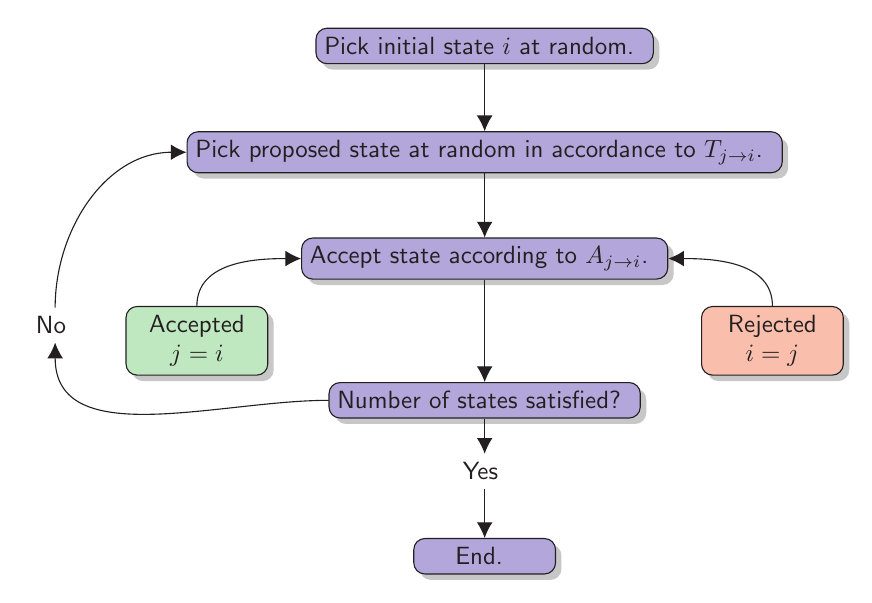
\begin{tikzpicture}[
            >={Latex[width=2mm,length=2mm]},
                base/.style = {rectangle, rounded corners, draw=black,
                            minimum width=2cm, minimum height=0.5cm, text
                            centered, font=\sffamily},
                basecode/.style = {rectangle, rounded corners, draw=black,
                            minimum width=2cm, minimum height=0.5cm, text
                            centered, font=\sffamily, align=left},
                activityStarts/.style = {base, fill=blue!30, drop shadow},
                startstop/.style = {base, fill=red!25, drop shadow},
                startstopcode/.style = {basecode, fill=red!25, drop shadow},
                activityRuns/.style = {base, fill=green!25, drop shadow},
                process/.style = {base, fill=white!15, font=\sffamily, drop shadow},
                processcode/.style = {basecode, fill=white!15, font=\sffamily, drop shadow},
            scale=0.8, 
            node distance=1.5cm, 
            every node/.style={fill=white, font=\sffamily, scale=0.9},
            align=center]
            \node (1) [activityStarts] {
                Pick initial state $i$ at random.
            };
            \node (2) [activityStarts, below of=1] {
                Pick proposed state at random in accordance to
                $\ufij{T}{j}{i}$.
            };
            \node (3) [activityStarts, below of=2] {
                Accept state according to $\ufij{A}{j}{i}$.
            };
            \node (a) [activityRuns, below left of=3, xshift=-3cm, yshift=-0.1cm] {
                Accepted \\
                $j = i$
            };
            \node (r) [startstop, below right of=3, xshift=3cm, yshift=-0.1cm] {
                Rejected \\
                $i = j$
            };
            \draw[<-] (3) to [out=180,in=90] (a);
            \draw[<-] (3) to [out=0,in=90] (r);
            \node (4) [activityStarts, below of=3, yshift=-0.5cm] {
                Number of states satisfied?
            };
            \node (yes) [below of=4, yshift=0.5cm] {
                Yes
            };
            \node (no) [above left of=4, xshift=-5cm] {
                No
            };
            \draw[->] (4) to [out=180, in=-90] (no);
            \draw[->] (no) to [out=90, in=180] (2);
            \node (5) [activityStarts, below of=yes, yshift=0.3cm] {
                End.
            };
            \draw[->] (1) -- (2);
            \draw[->] (2) -- (3);
            \draw[->] (3) -- (4);
            \draw[->] (4) -- (yes);
            \draw[->] (yes) -- (5);
        \end{tikzpicture}
    \end{figure}
\end{frame}

\section{Wavefunction}

{\setbeamercolor{palette primary}{fg=black, bg=white}
\begin{frame}[standout]{Wavefunction}
    $\phi_i(\blds{r}) = \sum\limits^L_{p=1} C_{pi}\chi_p(\blds{r})$
\end{frame}

{\setbeamercolor{palette primary}{fg=black, bg=white}
\begin{frame}[standout]{Wavefunction}
    $\phi_i(\blds{r}) = \sum\limits^L_{p=1} C_{pi}\color{red}{\chi_p(\blds{r})}$
\end{frame}

{\setbeamercolor{palette primary}{fg=black, bg=white}
\begin{frame}[standout]{Wavefunction: Integral Elements}
    $\Braket{\phi_i(\blds{r})|\phi_j(\blds{r})}$ \\ \vsp\vsp\vsp\vsp
    $\Braket{\phi_i(\blds{r})|x^k_d|\phi_j(\blds{r})}$ \\ \vsp\vsp\vsp\vsp
    $\Braket{\phi_i(\blds{r})|\nabla^2|\phi_j(\blds{r})}$ \\ \vsp\vsp\vsp\vsp
    $\Braket{\phi_i(\blds{r}_1)\phi_j(\blds{r}_2)|f_{12}|\phi_k(\blds{r}_1)\phi_l(\blds{r}_2)}$ \\
\end{frame}

\begin{frame}[fragile]{Wavefunction: Single-Well}
    \begin{itemize}
        \item Hermite Function: $\psi_n(\blds{r}) \equiv \prod\limits_d N_d
            H_{n_d}(\sqrt{\omega}x_d)\exp(-\frac{\omega}{2}x^2_d)$
    \end{itemize}
\end{frame}

\begin{frame}[fragile]{Wavefunction: Single-Well}
    \begin{itemize}
        \item Hermite Function: $\psi_n(\blds{r}) \equiv \prod\limits_d N_d
            H_{n_d}(\sqrt{\omega}x_d)\exp(-\frac{\omega}{2}x^2_d)$
        \item Solution in polar\footfullcite{anisimovas}
    \end{itemize}
\end{frame}

\begin{frame}[fragile]{Wavefunction: Single-Well}
    \begin{itemize}
        \item Hermite Function: $\psi_n(\blds{r}) \equiv \prod\limits_d N_d
            H_{n_d}(\sqrt{\omega}x_d)\exp(-\frac{\omega}{2}x^2_d)$
        \item Solution in polar\footfullcite{anisimovas}
        \item $\psi_n(\blds{r}) = \prod\limits_d N_d \sum\limits^{n_d}_{l=1}
            C^{\text{Hermite}}_{n_dl}
            g_l\left(\frac{\omega}{2},\blds{r},\blds{0}\right)$
    \end{itemize}
\end{frame}

\begin{frame}[fragile]{Wavefunction: Single-Well}
    \begin{itemize}
        \item Hermite Function: $\psi_n(\blds{r}) \equiv \prod\limits_d N_d
            H_{n_d}(\sqrt{\omega}x_d)\exp(-\frac{\omega}{2}x^2_d)$
        \item Solution in polar\footfullcite{anisimovas}
        \item $\psi_n(\blds{r}) = \prod\limits_d N_d \sum\limits^{n_d}_{l=1}
            C^{\text{Hermite}}_{n_dl}
            g_l\left(\frac{\omega}{2},\blds{r},\blds{0}\right)$
        \item Solution in Cartesian\footfullcite{HelgakerMolElcTheory} \\ \vspace{0.2cm} \hspace{1cm}
            \begin{minipage}[H]{0.5\textwidth}
                $\Braket{g_i(\blds{r})|g_j(\blds{r})}$ \vsp \\
                $\Braket{g_i(\blds{r})|x^k_d|g_j(\blds{r})}$ \vsp \\
                $\Braket{g_i(\blds{r})|\nabla^2|g_j(\blds{r})}$ \vsp \\
                $\Braket{g_i(\blds{r}_1)g_j(\blds{r}_2)|f_{12}|g_k(\blds{r}_1)g_l(\blds{r}_2)}$ \\
            \end{minipage}
    \end{itemize}
\end{frame}

\begin{frame}[fragile]{Wavefunction: Single-Well Integral Elements}
    \centering\footnotesize
    $\Braket{\psiHO_i|\psiHO_j} = N_i \delta_{ij}$ \\
    $\Braket{\psiHO_i|h^{\text{HO}}|\psiHO_j} =
    N_i\varepsilon^{\text{HO}}_i\delta_{ij}$ \\
    $\Braket{\psiHO_i\psiHO_j|\frac{1}{r_{12}}|\psiHO_k\psiHO_l} =
    \frac{aN_{ijkl}}{\sqrt{2\omega}}  \sum\limits^{ijkl}_{tuvw} H^{ijkl}_{tuvw}
    \suml{pq}{t+v,u+w} E^{tv}_pE^{uw}_q (-1)^q\xi_{p+q}\left(\frac{\omega}{2},
    \blds{0}\right)$
        \begin{equation*}
            \begin{aligned}
                E^{i+1,j}_t &= \frac{1}{2(\alpha + \beta)}E^{ij}_{t-1} -
                \frac{\beta}{\alpha+\beta}(A_x - B_x)E^{ij}_t +
                (t+1)E^{ij}_{t+1} \\
                E^{i,j+1}_t &= \frac{1}{2(\alpha + \beta)}E^{ij}_{t-1} -
                \frac{\alpha}{\alpha+\beta}(A_y - B_y)E^{ij}_t +
                (t+1)E^{ij}_{t+1} \\
                E^{00}_0 &= K_{AB}
            \end{aligned}
        \end{equation*}
        \begin{equation*}
            \begin{aligned}
                \xi^n_{t+1,u} &= t\xi^{n+1}_{t-1,u} + X_{AB}\xi^{n+1}_{t,u} \\
                \xi^n_{t,u+1} &= u\xi^{n+1}_{t,u-1} + Y_{AB}\xi^{n+1}_{t,u} \\
                \xi^n_{00} &= \left(\frac{-2\alpha\beta}{\alpha+\beta}\right)^n
                \zeta_n\left(\frac{\alpha\beta}{\alpha+\beta} R^2_{AB}\right) \\
                \zeta_n(x) &= \int\limits^1_{-1} \frac{u^{2n}}{\sqrt{1 -
                u^2}} \me^{-u^2x} \md u
            \end{aligned} \hspace{0.5cm}
            \begin{aligned}
                \xi^n_{t+1,u,v} &= t\xi^{n+1}_{t-1,u,v} + X_{AB}\xi^{n+1}_{t,u,v} \\
                \xi^n_{t,u+1,v} &= u\xi^{n+1}_{t,u-1,v} + Y_{AB}\xi^{n+1}_{t,u,v} \\
                \xi^n_{t,u,v+1} &= u\xi^{n+1}_{t,u,v-1} + Y_{AB}\xi^{n+1}_{t,u,v} \\
                \xi^n_{000} &= \left(-2\alpha\beta\right)^n
                \zeta_n\left(\frac{\alpha\beta}{\alpha+\beta} R^2_{AB}\right)
                \\
                \zeta_n(x) &= \int\limits^1_{-1} u^{2n} \me^{-u^2x} \md u
            \end{aligned}
        \end{equation*}
\end{frame}

\begin{frame}[fragile]{Wavefunction: Double-Well}
    \begin{itemize}
        \item Perturbation of harmonic oscillator: $\UDW(r) = \VHO(r) + \VDW_n(r)$
    \end{itemize}
\end{frame}

\begin{frame}[fragile]{Wavefunction: Double-Well}
    \begin{itemize}
        \item Perturbation of harmonic oscillator: $\UDW(r) = \VHO(r) + \VDW_n(r)$
        \item Expand in HO-functions: $\ket{\psiDW_p} = \sumll{l}C^{\text{DW}}_{lp}\ket{\psiHO_l}$
    \end{itemize}
\end{frame}

\begin{frame}[fragile]{Wavefunction: Double-Well}
    \begin{itemize}
        \item Perturbation of harmonic oscillator: $\UDW(r) = \VHO(r) + \VDW_n(r)$
        \item Expand in HO-functions: $\ket{\psiDW_p} = \sumll{l}C^{\text{DW}}_{lp}\ket{\psiHO_l}$
        \item Eigenvalue equation: $\blds{H}^{\text{DW}}\blds{C}^{\text{DW}} =
            \blds{\varepsilon^{\text{DW}}}\blds{C}^{\text{DW}}$
            \begin{itemize}
                \item $H^{\text{DW}}_{ij} = \veps^{\text{HO}}_i\delta_{ij} +
                    \Braket{\psiHO_i|\VDW_n|\psiHO_j}$
            \end{itemize}
    \end{itemize}
\end{frame}

\begin{frame}[fragile]{Wavefunction: Double-Well}
    \begin{itemize}
        \item Perturbation of harmonic oscillator: $\UDW(r) = \VHO(r) + \VDW_n(r)$
        \item Expand in HO-functions: $\ket{\psiDW_p} = \sumll{l}C^{\text{DW}}_{lp}\ket{\psiHO_l}$
        \item Eigenvalue equation: $\blds{H}^{\text{DW}}\blds{C}^{\text{DW}} =
            \blds{\varepsilon^{\text{DW}}}\blds{C}^{\text{DW}}$
            \begin{itemize}
                \item $H^{\text{DW}}_{ij} = \veps^{\text{HO}}_i\delta_{ij} +
                    \Braket{\psiHO_i|\VDW_n|\psiHO_j}$
            \end{itemize}
        \item Integral-Elements
        \begin{equation*}
            \footnotesize
            \begin{aligned}
                \Braket{\psiDW_p|\psiDW_q} &= \delta_{pq} \\
                \Braket{\psiDW_p|h^{\text{DW}}|\psiDW_q} &=
                \varepsilon^{\text{DW}}_p\delta_{pq} \\
                \Braket{\psiDW_p\psiDW_q|\frac{1}{r_{12}}|\psiDW_r\psiDW_s} &=
                \suml{tuvw}{ijkl} C^{\text{DW}}_{tp}C^{\text{DW}}_{uq}C^{\text{DW}}_{vr}C^{\text{DW}}_{ws}
                \Braket{\psiHO_t\psiHO_u|\frac{1}{r_{12}}|\psiHO_v\psiHO_w}
            \end{aligned}
        \end{equation*}
    \end{itemize}
\end{frame}

\begin{frame}[fragile]{Wavefunction: Slater-Jastrow}
    \begin{itemize}
        \item Slater determinant: $\psi_T =
            \det(\blds{\Phi(\blds{R};\blds{\alpha})})
            \xi(s)$
    \end{itemize}
\end{frame}

\begin{frame}[fragile]{Wavefunction: Slater-Jastrow}
    \begin{itemize}
        \item Slater determinant: $\psi_T =
            \det(\blds{\Phi(\blds{R};\blds{\alpha})}) \xi(s)$
        \item Modified Hermite: $\Phi_{ij} =
            \psi^{\text{HO}}_{n_j}(\sqrt{\alpha\omega}r_i) = \prod\limits_d N_d
            H_{n_d}(\sqrt{\alpha \omega}x_d)\me^{-\frac{\alpha\omega}{2}x^2_d}$
    \end{itemize}
\end{frame}

\begin{frame}[fragile]{Wavefunction: Slater-Jastrow}
    \begin{itemize}
        \item Slater determinant: $\psi_T =
            \det(\blds{\Phi(\blds{R};\blds{\alpha})}) \xi(s)$
        \item Modified Hermite: $\Phi_{ij} =
            \psi^{\text{HO}}_{n_j}(\sqrt{\alpha\omega}r_i) = \prod\limits_d N_d
            H_{n_d}(\sqrt{\alpha \omega}x_d)\me^{-\frac{\alpha\omega}{2}x^2_d}$
        \item Hartree-Fock: $\Phi_{ij} =
            \sum\limits_lC_{jl}\psi^{\text{HO}}_{n_l}\left(\sqrt{\omega}r_i\right)$
    \end{itemize}
\end{frame}

\begin{frame}[fragile]{Wavefunction: Slater-Jastrow}
    \begin{itemize}
        \item Slater determinant: $\psi_T =
            \det(\blds{\Phi(\blds{R};\blds{\alpha})}) \xi(s)$
        \item Modified Hermite: $\Phi_{ij} =
            \psi^{\text{HO}}_{n_j}(\sqrt{\alpha\omega}r_i) = \prod\limits_d N_d
            H_{n_d}(\sqrt{\alpha \omega}x_d)\me^{-\frac{\alpha\omega}{2}x^2_d}$
        \item Hartree-Fock: $\Phi_{ij} =
            \sum\limits_lC_{jl}\psi^{\text{HO}}_{n_l}\left(\sqrt{\omega}r_i\right)$
        \item Modified Hartree-Fock: $\Phi_{ij} =
            \sum\limits_lC_{jl}\psi^{\text{HO}}_{n_l}\left(\sqrt{\alpha\omega}r_i\right)$
    \end{itemize}
\end{frame}

\begin{frame}[fragile]{Wavefunction: Slater-Jastrow}
    \begin{itemize}
        \item Slater determinant: $\psi_T =
            \det(\blds{\Phi(\blds{R};\blds{\alpha})}) \xi(s)$
        \item Modified Hermite: $\Phi_{ij} =
            \psi^{\text{HO}}_{n_j}(\sqrt{\alpha\omega}r_i) = \prod\limits_d N_d
            H_{n_d}(\sqrt{\alpha \omega}x_d)\me^{-\frac{\alpha\omega}{2}x^2_d}$
        \item Hartree-Fock: $\Phi_{ij} =
            \sum\limits_lC_{jl}\psi^{\text{HO}}_{n_l}\left(\sqrt{\omega}r_i\right)$
        \item Modified Hartree-Fock: $\Phi_{ij} =
            \sum\limits_lC_{jl}\psi^{\text{HO}}_{n_l}\left(\sqrt{\alpha\omega}r_i\right)$
        \item Pad\'e-Jastrow: $J_{\text{Pad\'e}} = \prod\limits_{i<j}
            \me^{\frac{a_{ij} r_{ij}}{1 + \beta r_{ij}}}$
    \end{itemize}
\end{frame}

\begin{frame}[fragile]{Wavefunction: Slater-Jastrow}
    \begin{itemize}
        \item Slater determinant: $\psi_T =
            \det(\blds{\Phi(\blds{R};\blds{\alpha})}) \xi(s)$
        \item Modified Hermite: $\Phi_{ij} =
            \psi^{\text{HO}}_{n_j}(\sqrt{\alpha\omega}r_i) = \prod\limits_d N_d
            H_{n_d}(\sqrt{\alpha \omega}x_d)\me^{-\frac{\alpha\omega}{2}x^2_d}$
        \item Hartree-Fock: $\Phi_{ij} =
            \sum\limits_lC_{jl}\psi^{\text{HO}}_{n_l}\left(\sqrt{\omega}r_i\right)$
        \item Modified Hartree-Fock: $\Phi_{ij} =
            \sum\limits_lC_{jl}\psi^{\text{HO}}_{n_l}\left(\sqrt{\alpha\omega}r_i\right)$
        \item Pad\'e-Jastrow: $J_{\text{Pad\'e}} = \prod\limits_{i<j}
            \me^{\frac{a_{ij} r_{ij}}{1 + \beta r_{ij}}}$
        \item NQS: $J_{\text{NQS}} = \me^{-\suml{i=1}{N} \frac{\left(\bm{r}_i -
            \bm{a}_i\right)^2}{2\sigma^2}}\prod\limits^{M}_j \left(1 + \me^{b_j
            + \suml{i=1}{N}\suml{d=1}{D}
            \frac{x^{(d)}_iw_{i+d,j}}{\sigma^2}}\right)$
    \end{itemize}
\end{frame}

\begin{frame}[fragile]{Wavefunction: Slater-Jastrow}
    \begin{itemize}
        \item Slater determinant: $\psi_T =
            \det(\blds{\Phi(\blds{R};\blds{\alpha})}) \xi(s)$
        \item Modified Hermite: $\Phi_{ij} =
            \psi^{\text{HO}}_{n_j}(\sqrt{\alpha\omega}r_i) = \prod\limits_d N_d
            H_{n_d}(\sqrt{\alpha \omega}x_d)\me^{-\frac{\alpha\omega}{2}x^2_d}$
        \item Hartree-Fock: $\Phi_{ij} =
            \sum\limits_lC_{jl}\psi^{\text{HO}}_{n_l}\left(\sqrt{\omega}r_i\right)$
        \item Modified Hartree-Fock: $\Phi_{ij} =
            \sum\limits_lC_{jl}\psi^{\text{HO}}_{n_l}\left(\sqrt{\alpha\omega}r_i\right)$
        \item Pad\'e-Jastrow: $J_{\text{Pad\'e}} = \prod\limits_{i<j}
            \me^{\frac{a_{ij} r_{ij}}{1 + \beta r_{ij}}}$
        \item NQS: $J_{\text{NQS}} = \me^{-\suml{i=1}{N} \frac{\left(\bm{r}_i -
            \bm{a}_i\right)^2}{2\sigma^2}}\prod\limits^{M}_j \left(1 + \me^{b_j
            + \suml{i=1}{N}\suml{d=1}{D}
            \frac{x^{(d)}_iw_{i+d,j}}{\sigma^2}}\right)$
        \item Pad\'e-NQS: $J = J_{\text{Pad\'e}}J_{\text{NQS}}$
    \end{itemize}
\end{frame}

\begin{frame}[fragile]{Wavefunction: Slater-Jastrow}
    \begin{itemize}
        \item Slater determinant: $\psi =
            \det(\blds{\Phi(\blds{R};\blds{\alpha})}) \xi(s)$
        \item Modified Hermite: $\Phi_{ij} =
            \psi^{\text{HO}}_{n_j}(\sqrt{\alpha\omega}r_i) = \prod\limits_d N_d
            H_{n_d}(\sqrt{\alpha \omega}x_d)\me^{-\frac{\alpha\omega}{2}x^2_d}$
        \item Hartree-Fock: $\Phi_{ij} =
            \sum\limits_lC_{jl}\psi^{\text{HO}}_{n_l}\left(\sqrt{\omega}r_i\right)$
        \item Modified Hartree-Fock: $\Phi_{ij} =
            \sum\limits_lC_{jl}\psi^{\text{HO}}_{n_l}\left(\sqrt{\alpha\omega}r_i\right)$
        \item Pad\'e-Jastrow: $J_{\text{Pad\'e}} = \prod\limits_{i<j}
            \me^{\frac{a_{ij} r_{ij}}{1 + \beta r_{ij}}}$
        \item NQS: $J_{\text{NQS}} = \me^{-\suml{i=1}{N} \frac{\left(\bm{r}_i -
            \bm{a}_i\right)^2}{2\sigma^2}}\prod\limits^{M}_j \left(1 + \me^{b_j
            + \suml{i=1}{N}\suml{d=1}{D}
            \frac{x^{(d)}_iw_{i+d,j}}{\sigma^2}}\right)$
        \item Pad\'e-NQS: $J = J_{\text{Pad\'e}}J_{\text{NQS}}$
    \end{itemize}
\end{frame}

\section{Implementation}

\begin{frame}[fragile]{Implementation}
\end{frame}

\begin{frame}[fragile]{Implementation}
    \begin{itemize}
        \item \CC and Eigen
    \end{itemize}
\end{frame}

\begin{frame}[fragile]{Implementation}
    \begin{itemize}
        \item \CC and Eigen
            \begin{itemize}
                \item Performance
            \end{itemize}
    \end{itemize}
\end{frame}

\begin{frame}[fragile]{Implementation}
    \begin{itemize}
        \item \CC and Eigen
            \begin{itemize}
                \item Performance
                \item Generalization
            \end{itemize}
    \end{itemize}
\end{frame}

\begin{frame}[fragile]{Implementation}
    \begin{itemize}
        \item \CC and Eigen
            \begin{itemize}
                \item Performance
                \item Generalization
            \end{itemize}
        \item Python
    \end{itemize}
\end{frame}

\begin{frame}[fragile]{Implementation}
    \begin{itemize}
        \item \CC and Eigen
            \begin{itemize}
                \item Performance
                \item Generalization
            \end{itemize}
        \item Python
            \begin{itemize}
               \item Generate \CC code 
            \end{itemize}
    \end{itemize}
\end{frame}

\begin{frame}[fragile]{Implementation: Cartesian}
    \begin{figure}[H]
        \centering
        \begin{tikzpicture}[scale=1.0]
            \draw (-1,0) -- (1,0);
            \node at (-0.5,0) [draw,circle,fill=red,scale=0.6] {};
            \node at (0.5,0) [draw,circle,fill=red,scale=0.6] {};
            \draw[blue, ->] (-0.5,-0.5) -- (-0.5,0.5);
            \draw[blue, <-] (0.5,-0.5) -- (0.5,0.5);
            \node[text width=2.2cm, align=center] at (0,-1) {\footnotesize{$(0,0)$}};
            \draw (-2.5,2) -- (-0.5,2);
            \node at (-2.0,2) [draw,circle,fill=red,scale=0.6] {};
            \node at (-1.0,2) [draw,circle,fill=red,scale=0.6] {};
            \draw[blue, ->] (-2.0,1.5) -- (-2.0,2.5);
            \draw[blue, <-] (-1.0,1.5) -- (-1.0,2.5);
            \node[text width=2.2cm, align=center] at (-1.5,1) {\footnotesize{$(1,0)$}};
            \draw (0.5,2) -- (2.5,2);
            \node at (1.0,2) [draw,circle,fill=red,scale=0.6] {};
            \node at (2.0,2) [draw,circle,fill=red,scale=0.6] {};
            \draw[blue, <-] (1.0,1.5) -- (1.0,2.5);
            \draw[blue, ->] (2.0,1.5) -- (2.0,2.5);
            \node[text width=2.2cm, align=center] at (1.5,1) {\footnotesize{$(0,1)$}};
            \draw (-4.5,4) -- (-2.5,4);
            \node at (-4.0,4) [draw,circle,fill=red,scale=0.6] {};
            \node at (-3.0,4) [draw,circle,fill=red,scale=0.6] {};
            \draw[blue, ->] (-4.0,3.5) -- (-4.0,4.5);
            \draw[blue, <-] (-3.0,3.5) -- (-3.0,4.5);
            \node[text width=2.2cm, align=center] at (-3.5,3) {\footnotesize{$(2,0)$}};
            \draw (-1,4) -- (1,4);
            \node at (-0.5,4) [draw,circle,fill=red,scale=0.6] {};
            \node at (0.5,4) [draw,circle,fill=red,scale=0.6] {};
            \draw[blue, ->] (-0.5,3.5) -- (-0.5,4.5);
            \draw[blue, <-] (0.5,3.5) -- (0.5,4.5);
            \node[text width=2.2cm, align=center] at (0,3) {\footnotesize{$(1,1)$}};
            \draw (4.5,4) -- (2.5,4);
            \node at (4.0,4) [draw,circle,fill=red,scale=0.6] {};
            \node at (3.0,4) [draw,circle,fill=red,scale=0.6] {};
            \draw[blue, ->] (4.0,3.5) -- (4.0,4.5);
            \draw[blue, <-] (3.0,3.5) -- (3.0,4.5);
            \node[text width=2.2cm, align=center] at (3.5,3) {\footnotesize{$(0,2)$}};
        \end{tikzpicture}
    \end{figure}
\end{frame}

\begin{frame}[fragile]{Implementation: Hartree-Fock}
    \begin{figure}[H]
        \centering
        \begin{tikzpicture}[
            >={Latex[width=2mm,length=2mm]},
                base/.style = {rectangle, rounded corners, draw=black,
                            minimum width=2cm, minimum height=0.5cm, text
                            centered, font=\sffamily},
                basecode/.style = {rectangle, rounded corners, draw=black,
                            minimum width=2cm, minimum height=0.5cm, text
                            centered, font=\sffamily, align=left},
                activityStarts/.style = {base, fill=blue!30, drop shadow},
                startstop/.style = {base, fill=red!25, drop shadow},
                startstopcode/.style = {basecode, fill=red!25, drop shadow},
                activityRuns/.style = {base, fill=green!25, drop shadow},
                process/.style = {base, fill=white!15, font=\sffamily, drop shadow},
                processcode/.style = {basecode, fill=white!15, font=\sffamily, drop shadow},
            scale=0.8, 
            node distance=1.5cm, 
            every node/.style={fill=white, font=\sffamily, scale=0.49},
            align=center]
            \node (Hexpander) [processcode] {
                \hltexttt{Hexpander}
            };
            \node (GaussianQuadrature) [processcode, left of=Hexpander, xshift=-3cm] {
                \hltexttt{GaussianQuadrature}
            };
            \node (Cartesian) [processcode, below of=HartreeFockSolver] {
                \hltexttt{Cartesian}
            };
            \node (Hermite) [processcode, below of=Cartesian] {
                \hltexttt{Hermite}
            };
            \node (HartreeFockSolver) [processcode, below of=Hermite] {
                \hltexttt{HartreeFockSolver}
            };
            \node (GaussianIntegrals) [processcode, above right of=HartreeFockSolver, xshift=4cm] {
                \hltexttt{GaussianIntegrals}
            };
            \node (DoubleWell) [processcode, below right of=HartreeFockSolver, xshift=4cm] {
                \hltexttt{DoubleWell}
            };
            \node (DWC) [processcode, below of=HartreeFockSolver] {
                \hltexttt{DWC}
            };
            \draw[->] (GaussianQuadrature) -- (Hexpander);
            \draw[->] (Hexpander) to [out=0, in=90] (GaussianIntegrals);
            \draw[->] (Cartesian) to [out=0, in=90] (GaussianIntegrals);
            \draw[->] (Hermite) to [out=0, in=90] (GaussianIntegrals);
            \draw[->] (HartreeFockSolver) to [out=0, in=180] (GaussianIntegrals);
            \draw[->] (HartreeFockSolver) to [out=0, in=180] (DoubleWell);
            \draw[->] (DWC) to [out=0, in=180] (DoubleWell);
            \draw[->] (GaussianIntegrals) -- (DoubleWell);
        \end{tikzpicture}
    \end{figure}
\end{frame}

\begin{frame}[fragile]{Implementation: Hartree-Fock}
    \begin{figure}[H]
        \centering
        \begin{tikzpicture}[
            >={Latex[width=2mm,length=2mm]},
                base/.style = {rectangle, rounded corners, draw=black,
                            minimum width=2cm, minimum height=0.5cm, text
                            centered, font=\sffamily},
                basecode/.style = {rectangle, rounded corners, draw=black,
                            minimum width=2cm, minimum height=0.5cm, text
                            centered, font=\sffamily, align=left},
                activityStarts/.style = {base, fill=blue!30, drop shadow},
                startstop/.style = {base, fill=red!25, drop shadow},
                startstopcode/.style = {basecode, fill=red!25, drop shadow},
                activityRuns/.style = {base, fill=green!25, drop shadow},
                process/.style = {base, fill=white!15, font=\sffamily, drop shadow},
                processcode/.style = {basecode, fill=white!15, font=\sffamily, drop shadow},
            scale=0.8, 
            node distance=1.5cm, 
            every node/.style={fill=white, font=\sffamily, scale=0.49},
            align=center]
            \node (_Hexpander) [processcode] {
                \hltexttt{Hexpander}
            };
            \node (_GaussianQuadrature) [processcode, left of=_Hexpander, xshift=-3cm] {
                \hltexttt{GaussianQuadrature}
            };
            \node (_Cartesian) [processcode, below of=_HartreeFockSolver] {
                \hltexttt{Cartesian}
            };
            \node (_Hermite) [processcode, below of=_Cartesian] {
                \hltexttt{Hermite}
            };
            \node (_HartreeFockSolver) [processcode, below of=_Hermite] {
                \hltexttt{HartreeFockSolver}
            };
            \node (_GaussianIntegrals) [processcode, above right of=_HartreeFockSolver, xshift=4cm] {
                \hltexttt{GaussianIntegrals}
            };
            \node (_DoubleWell) [processcode, below right of=_HartreeFockSolver, xshift=4cm] {
                \hltexttt{DoubleWell}
            };
            \node (_DWC) [processcode, below of=_HartreeFockSolver] {
                \hltexttt{DWC}
            };
            \draw[->] (_GaussianQuadrature) -- (_Hexpander);
            \draw[->] (_Hexpander) to [out=0, in=90] (_GaussianIntegrals);
            \draw[->] (_Cartesian) to [out=0, in=90] (_GaussianIntegrals);
            \draw[->] (_Hermite) to [out=0, in=90] (_GaussianIntegrals);
            \draw[->] (_HartreeFockSolver) to [out=0, in=180] (_GaussianIntegrals);
            \draw[->] (_HartreeFockSolver) to [out=0, in=180] (_DoubleWell);
            \draw[->] (_DWC) to [out=0, in=180] (_DoubleWell);
            \draw[->] (_GaussianIntegrals) -- (_DoubleWell);
        \end{tikzpicture}
    \end{figure}
    \begin{itemize}
        \item Parallelization
            \begin{itemize}
                \item Two-body element is computationally expensive
                \item $S_i = \suml{j=0}{P_i} \prod\limits_d (n_{j_d}+1)$
            \end{itemize}
    \end{itemize}
\end{frame}

\begin{frame}[fragile]{Implementation: Hartree-Fock}
    \begin{figure}[H]
        \centering
        \begin{tikzpicture}[
            >={Latex[width=2mm,length=2mm]},
                base/.style = {rectangle, rounded corners, draw=black,
                            minimum width=2cm, minimum height=0.5cm, text
                            centered, font=\sffamily},
                basecode/.style = {rectangle, rounded corners, draw=black,
                            minimum width=2cm, minimum height=0.5cm, text
                            centered, font=\sffamily, align=left},
                activityStarts/.style = {base, fill=blue!30, drop shadow},
                startstop/.style = {base, fill=red!25, drop shadow},
                startstopcode/.style = {basecode, fill=red!25, drop shadow},
                activityRuns/.style = {base, fill=green!25, drop shadow},
                process/.style = {base, fill=white!15, font=\sffamily, drop shadow},
                processcode/.style = {basecode, fill=white!15, font=\sffamily, drop shadow},
            scale=0.8, 
            node distance=1.5cm, 
            every node/.style={fill=white, font=\sffamily, scale=0.49},
            align=center]
            \node (__Hexpander) [processcode] {
                \hltexttt{Hexpander}
            };
            \node (__GaussianQuadrature) [processcode, left of=__Hexpander, xshift=-3cm] {
                \hltexttt{GaussianQuadrature}
            };
            \node (__Cartesian) [processcode, below of=__HartreeFockSolver] {
                \hltexttt{Cartesian}
            };
            \node (__Hermite) [processcode, below of=__Cartesian] {
                \hltexttt{Hermite}
            };
            \node (__HartreeFockSolver) [processcode, below of=__Hermite] {
                \hltexttt{HartreeFockSolver}
            };
            \node (__GaussianIntegrals) [processcode, above right of=__HartreeFockSolver, xshift=4cm] {
                \hltexttt{GaussianIntegrals}
            };
            \node (__DoubleWell) [processcode, below right of=__HartreeFockSolver, xshift=4cm] {
                \hltexttt{DoubleWell}
            };
            \node (__DWC) [processcode, below of=__HartreeFockSolver] {
                \hltexttt{DWC}
            };
            \draw[->] (__GaussianQuadrature) -- (__Hexpander);
            \draw[->] (__Hexpander) to [out=0, in=90] (__GaussianIntegrals);
            \draw[->] (__Cartesian) to [out=0, in=90] (__GaussianIntegrals);
            \draw[->] (__Hermite) to [out=0, in=90] (__GaussianIntegrals);
            \draw[->] (__HartreeFockSolver) to [out=0, in=180] (__GaussianIntegrals);
            \draw[->] (__HartreeFockSolver) to [out=0, in=180] (__DoubleWell);
            \draw[->] (__DWC) to [out=0, in=180] (__DoubleWell);
            \draw[->] (__GaussianIntegrals) -- (__DoubleWell);
        \end{tikzpicture}
    \end{figure}
    \begin{itemize}
        \item Parallelization
            \begin{itemize}
                \item Two-body element is computationally expensive
                \item $S_i = \suml{j=0}{P_i} \prod\limits_d (n_{j_d}+1)$
            \end{itemize}
        \item Hartree-Fock algorithm only run on one process
    \end{itemize}
\end{frame}

\begin{frame}[fragile]{Implementation: Hartree-Fock}
    \begin{figure}[H]
        \centering
        \begin{tikzpicture}[
            >={Latex[width=2mm,length=2mm]},
                base/.style = {rectangle, rounded corners, draw=black,
                            minimum width=2cm, minimum height=0.5cm, text
                            centered, font=\sffamily},
                basecode/.style = {rectangle, rounded corners, draw=black,
                            minimum width=2cm, minimum height=0.5cm, text
                            centered, font=\sffamily, align=left},
                activityStarts/.style = {base, fill=blue!30, drop shadow},
                startstop/.style = {base, fill=red!25, drop shadow},
                startstopcode/.style = {basecode, fill=red!25, drop shadow},
                activityRuns/.style = {base, fill=green!25, drop shadow},
                process/.style = {base, fill=white!15, font=\sffamily, drop shadow},
                processcode/.style = {basecode, fill=white!15, font=\sffamily, drop shadow},
            scale=0.8, 
            node distance=1.5cm, 
            every node/.style={fill=white, font=\sffamily, scale=0.49},
            align=center]
            \node (___Hexpander) [processcode] {
                \hltexttt{Hexpander}
            };
            \node (___GaussianQuadrature) [processcode, left of=___Hexpander, xshift=-3cm] {
                \hltexttt{GaussianQuadrature}
            };
            \node (___Cartesian) [processcode, below of=___HartreeFockSolver] {
                \hltexttt{Cartesian}
            };
            \node (___Hermite) [processcode, below of=___Cartesian] {
                \hltexttt{Hermite}
            };
            \node (___HartreeFockSolver) [processcode, below of=___Hermite] {
                \hltexttt{HartreeFockSolver}
            };
            \node (___GaussianIntegrals) [processcode, above right of=___HartreeFockSolver, xshift=4cm] {
                \hltexttt{GaussianIntegrals}
            };
            \node (___DoubleWell) [processcode, below right of=___HartreeFockSolver, xshift=4cm] {
                \hltexttt{DoubleWell}
            };
            \node (___DWC) [processcode, below of=___HartreeFockSolver] {
                \hltexttt{DWC}
            };
            \draw[->] (___GaussianQuadrature) -- (___Hexpander);
            \draw[->] (___Hexpander) to [out=0, in=90] (___GaussianIntegrals);
            \draw[->] (___Cartesian) to [out=0, in=90] (___GaussianIntegrals);
            \draw[->] (___Hermite) to [out=0, in=90] (___GaussianIntegrals);
            \draw[->] (___HartreeFockSolver) to [out=0, in=180] (___GaussianIntegrals);
            \draw[->] (___HartreeFockSolver) to [out=0, in=180] (___DoubleWell);
            \draw[->] (___DWC) to [out=0, in=180] (___DoubleWell);
            \draw[->] (___GaussianIntegrals) -- (___DoubleWell);
        \end{tikzpicture}
    \end{figure}
    \begin{itemize}
        \item Parallelization
            \begin{itemize}
                \item Two-body element is computationally expensive
                \item $S_i = \suml{j=0}{P_i} \prod\limits_d (n_{j_d}+1)$
            \end{itemize}
        \item Hartree-Fock algorithm only run on one process
        \item Tabulation of Two-Body matrix
    \end{itemize}
\end{frame}

\begin{frame}[fragile]{Implementation: Variational Monte-Carlo}
\end{frame}

\section{Summary and Conclusion}

{\setbeamercolor{palette primary}{fg=orange, bg=white}
\begin{frame}[standout]
  Questions?
\end{frame}
}

\appendix

{\setbeamercolor{palette primary}{fg=orange, bg=white}
\begin{frame}[standout]{Questions}
    Questions?
\end{frame}

\end{document}
